\vspace{1em}

\usetikzlibrary{graphs, positioning, quotes, shapes.geometric}

\begin{document}
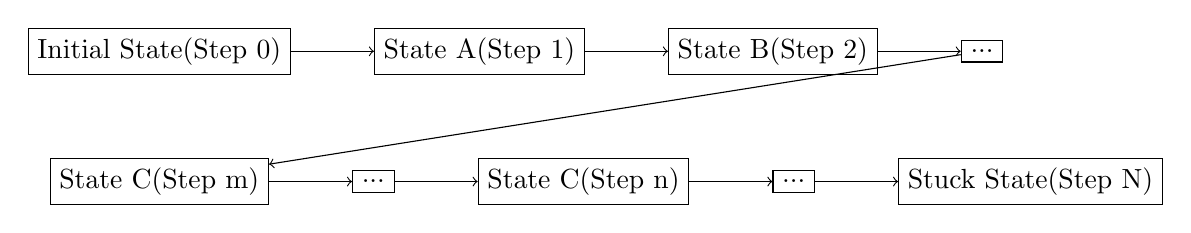
\begin{tikzpicture}[node distance=10pt]
    \node[draw]                           (State 0)  {Initial State(Step 0)};
    \node[draw, right=30pt of State 0]    (State 1)  {State A(Step 1)};
    \node[draw, right=30pt of State 1]    (State 2)  {State B(Step 2)};
    \node[draw, right=30pt of State 2]    (State 3)  {...};

    \node[draw, below=30pt of State 0]    (State 4)  {State C(Step m)};
    \node[draw, right=30pt of State 4]    (State 5)  {...};
    \node[draw, right=30pt of State 5]    (State 6)  {State C(Step n)};
    \node[draw, right=30pt of State 6]    (State 7)  {...};
    \node[draw, right=30pt of State 7]    (State 8)  {Stuck State(Step N)};
    
    \graph{
        (State 0) -> (State 1) -> (State 2) -> (State 3) -> (State 4) -> (State 5) -> (State 6) -> (State 7) -> (State 8);
    };
\end{tikzpicture}